\documentclass{article}
% The file ijcai15.sty is the style file for IJCAI-15 (same as ijcai07.sty).
\usepackage{ijcai15}

% Use the postscript times font!
\usepackage{times}
\usepackage{helvet}
\usepackage{courier}
\usepackage{bm}
\usepackage{amsmath}
\usepackage{cases}
\usepackage{multirow}
\usepackage{algorithm}
\usepackage{algorithmic}
\usepackage{booktabs}
\usepackage{graphicx}


\begin{document}
\section{Figures}

\begin{figure} [htbp]
\centering
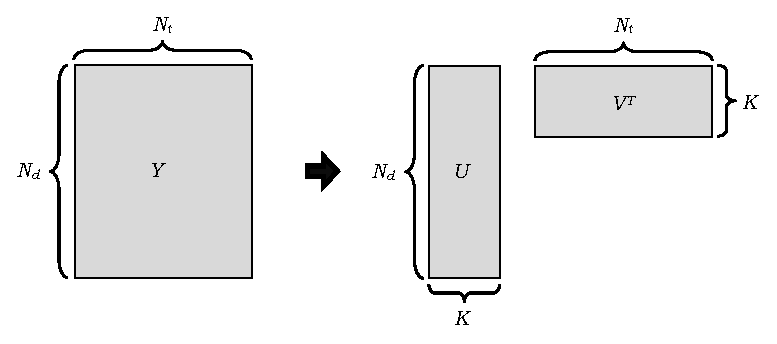
\includegraphics[width=8cm]{fig_tmf_matrix_new}
\caption{Schematic figure of matrix factorization.}\label{fig_tmf_matrix}
\end{figure}

\begin{figure} [htbp]
\centering
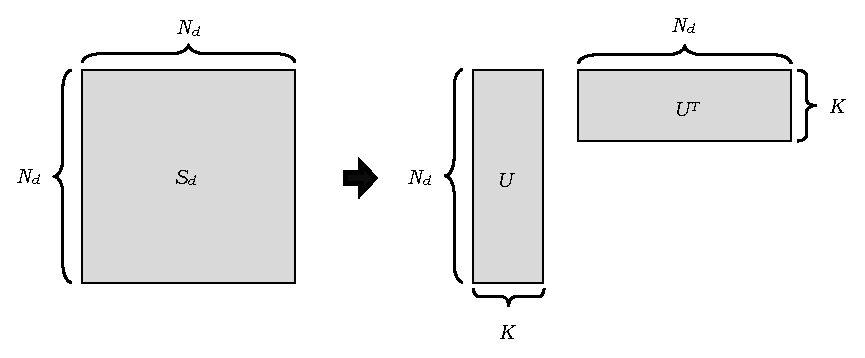
\includegraphics[width=8cm]{fig_cmf_sim_drug}
\caption{Schematic figure of drug similarity approximation.}\label{fig_cmf_sim_drug}
\end{figure}

\begin{figure} [htbp]
\centering
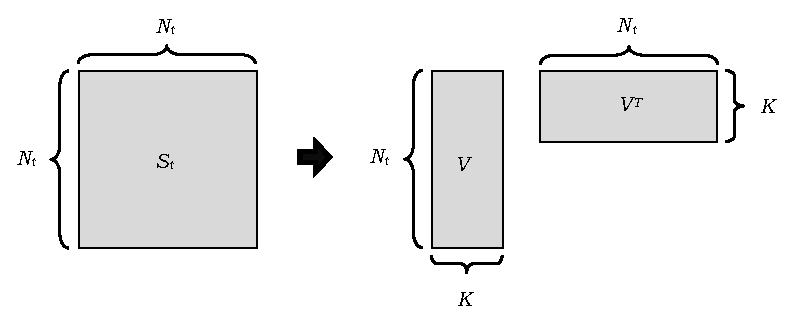
\includegraphics[width=8cm]{fig_cmf_sim_target}
\caption{Schematic figure of target similarity approximation.}\label{fig_cmf_sim_target}
\end{figure}

\begin{figure} [htbp]
\centering
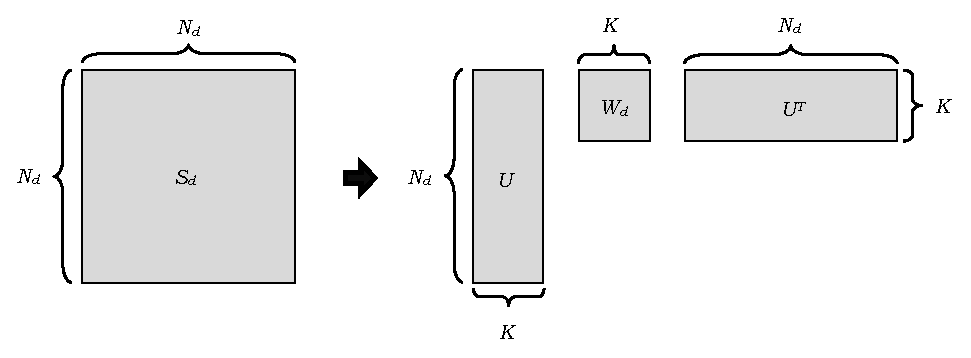
\includegraphics[width=8cm]{fig_tmf_sim_drug_new}
\caption{Schematic figure of drug similarity approximation.}\label{fig_tmf_sim_drug}
\end{figure}

\begin{figure} [htbp]
\centering
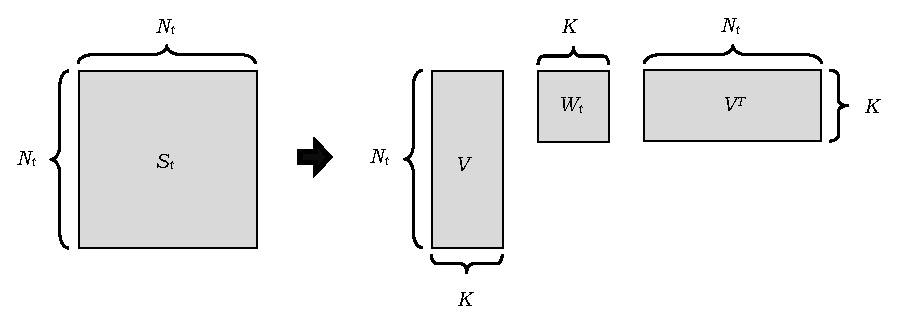
\includegraphics[width=8cm]{fig_tmf_sim_target_new}
\caption{Schematic figure of target similarity approximation.}\label{fig_tmf_sim_target}
\end{figure}

\begin{figure} [htbp]
\centering
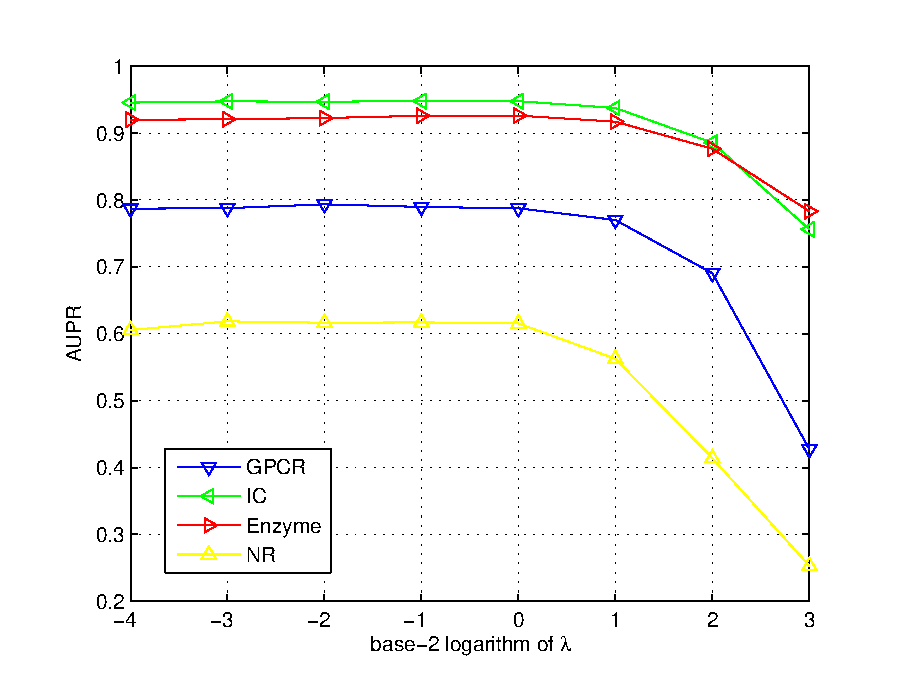
\includegraphics[width=8cm]{effect_lambda}
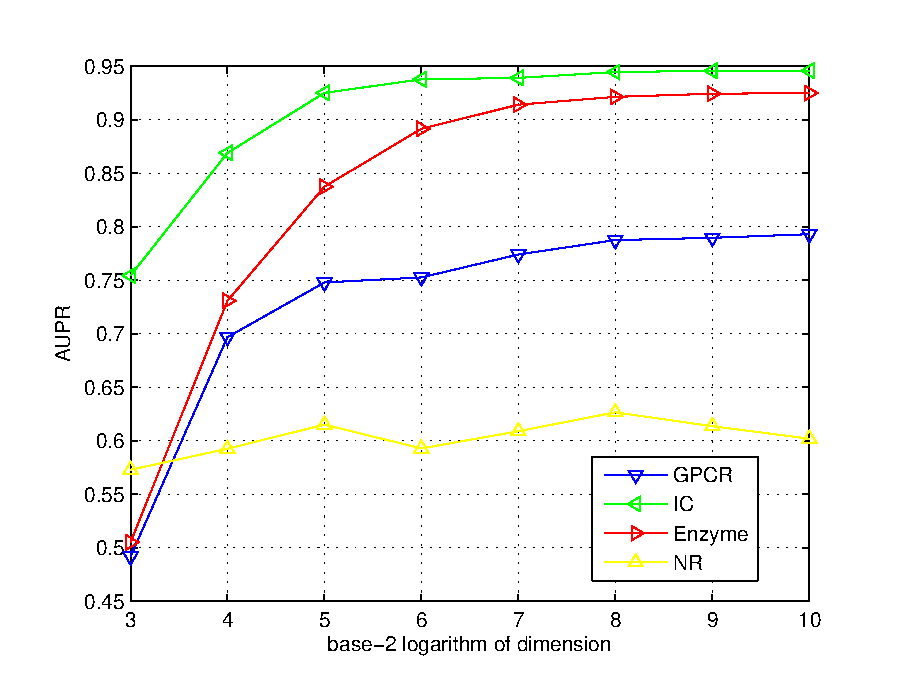
\includegraphics[width=8cm]{effect_dim}
\caption{effect of lambda and dim.}\label{effect_lambda_dim}
\end{figure}

\begin{figure} [htbp]
\centering
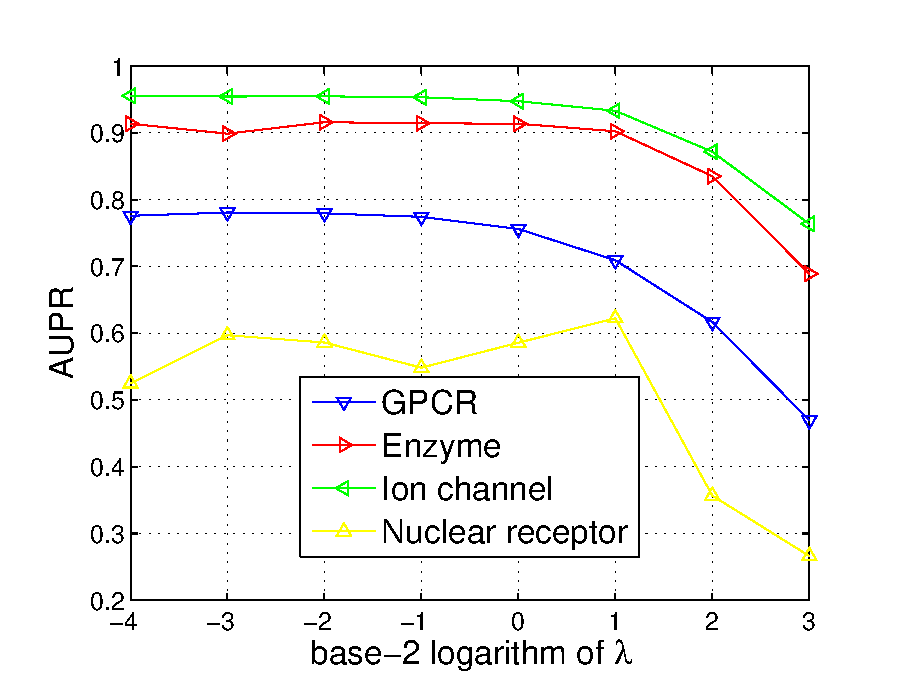
\includegraphics[width=8cm]{mstmf_w_effect_lambda}
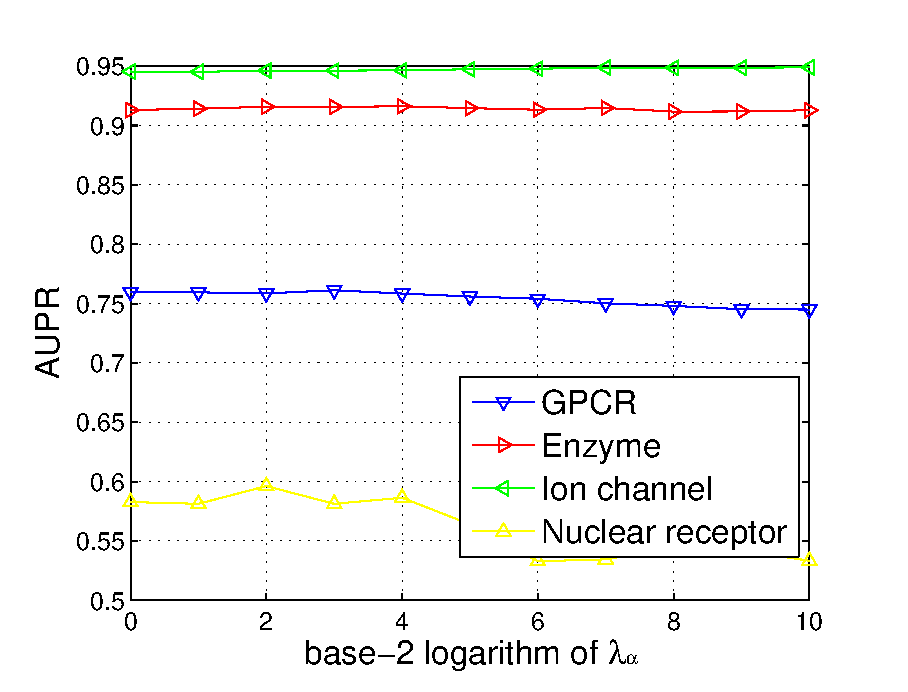
\includegraphics[width=8cm]{mstmf_w_effect_lambdaA}
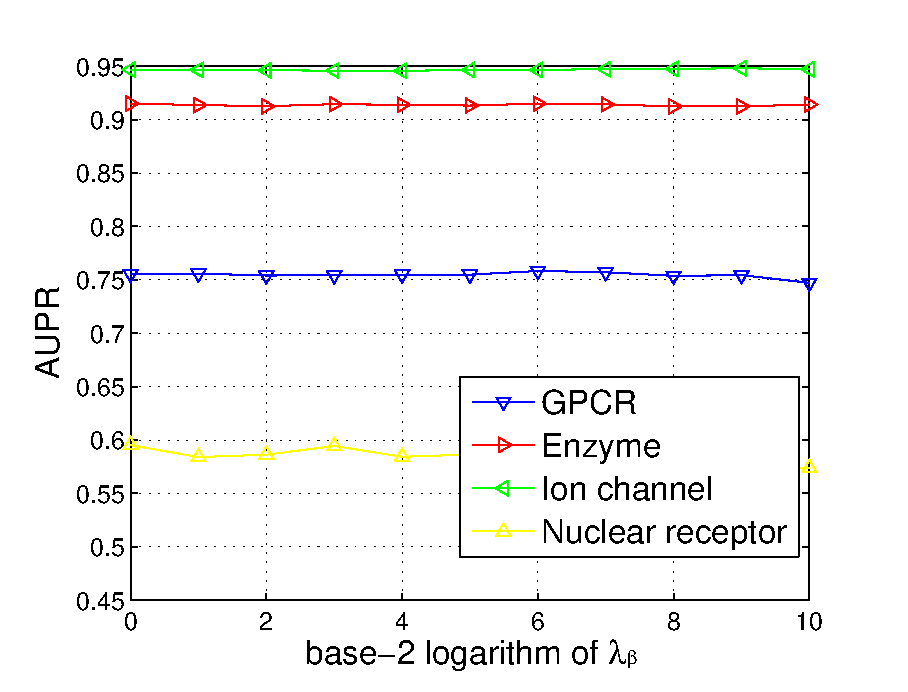
\includegraphics[width=8cm]{mstmf_w_effect_lambdaB}
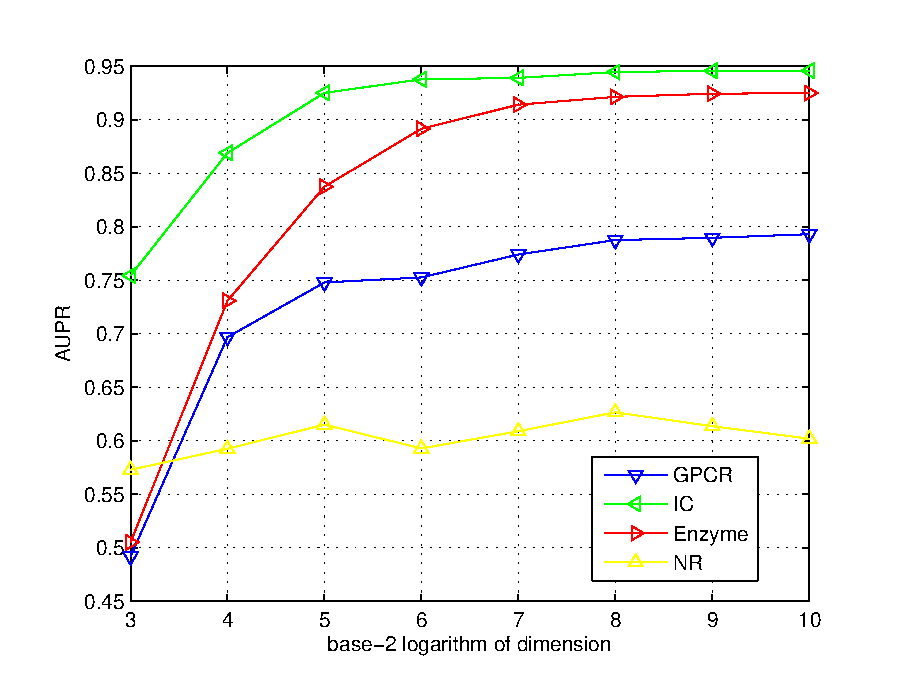
\includegraphics[width=8cm]{effect_dim}
\caption{effect of lambda and dim.}\label{effect_lambda_dim}
\end{figure}

\section{Why only pair prediction}
I think my supervisor has answered this question in the email. 

\section{T test}
See table\ref{results_comp_with_other_methods}.
We computed the p value for each method with the best method.

%---table results_comp_with_other_methods
\begin{table*}[htbp]
\caption{AUPR values obtained by 5$\times$10-fold cross validation. The highest AUPR value for each column is highlighted in boldface. }\label{results_comp_with_other_methods}
\centering
\leftline{Pair prediction}
\begin{tabular}{lllll}
\toprule
Methods & GPCR & Enzyme & IC & NR\\
\midrule
BLM & 0.666(1.20e-28) & 0.830(5.54e-41) & 0.847(4.74e-38) & 0.509(7.26e-08) \\
PKM & 0.401(2.14e-22) & 0.633(1.27e-47)  & 0.617(1.11e-47) & 0.499(9.14e-12) \\
LapRLS & 0.639(3.35e-31) & 0.826(4.50e-45) & 0.804(1.28e-37) & 0.539(3.08e-08)\\
NetLapRLS & 0.660(7.22e-30) & 0.840(5.41e-44) & 0.848(3.55e-32) & 0.545(2.18e-08)\\
GIP	 & 0.710(7.08e-25) & 0.869(5.68e-35) & 0.889(9.37e-30) & 0.596(3.47e-04)\\
KBMF2K & 0.686(9.83e-25) & 0.796(4.01e-43) & 0.876(3.29e-28) & 0.508(9.13e-10) \\
CMF & 0.739(5.90e-20) & 0.896(1.28e-32) & 0.938(4.21e-14) & 0.568(3.80e-05)\\
\textbf{TMF} & \textbf{0.794}(2.11e-01) & \textbf{0.913}(1.67e-19) & \textbf{0.945}(5.53e-09) & \textbf{0.611}(3.02e-03) \\ 
\midrule
MSCMF & 0.743(7.16e-18) & 0.913(4.16e-21) & 0.938(8.43e-13) & 0.562(1.71e-05) \\
\textbf{MSTMF} & 0.787(3.16e-05) & \textbf{0.927} & 0.949(5.00e-03) & \textbf{0.658} \\
\textbf{MSTMF-weight} & \textbf{0.796} & 0.925(1.75e-06) & \textbf{0.951} & 0.645(1.63e-01)\\
\bottomrule
\end{tabular} \\
\end{table*}

\section{Table of weights}

%---table of weights
\begin{table}[h]
\caption{A typical case of resultant similarity weights under
pair prediction.}\label{weight_table}
(a)similarities over drugs \\
\begin{tabular}{lrrrr}
\toprule
 & \textit{GPCR} & \textit{Enzyme} & \textit{IC} & \textit{NR} \\
\midrule
CS & 0.5477 & 0.5367 & 0.6231 & 0.6077 \\
ATC& 0.4523 & 0.4633 & 0.3769 & 0.3923\\
\bottomrule
\end{tabular}

(b)similarities over targets \\
\begin{tabular}{lrrrr}
\toprule
 & \textit{GPCR} & \textit{Enzyme} & \textit{IC} & \textit{NR} \\
\midrule
GS & 0.8350 & 0.8436 & 0.6220 & 0.9589 \\
GO(MF)& 0.1650 & 0.1564 & 0.3780 & 0.0411\\
\bottomrule
\end{tabular}

\end{table}

This is one case of similarity weights under pair prediction of MSTMF-weight. We can see that it is quite different from MSCMF compare to Table3 in the KDD2013 paper. Because the weights are sensitive to the choosing of $\lambda_\alpha$ and $\lambda_\beta$, so different cases may have quite different weights.

\end{document}